\documentclass[a4paper]{article}

\usepackage{amsmath,longtable,fancyhdr,booktabs,multirow,graphicx,float}
\usepackage{amssymb,xcolor,amsthm}
\usepackage{color}
\usepackage[colorlinks,
       %     linkcolor=black,
       %     anchorcolor=blue,
       %     citecolor=green
           ]{hyperref}
\usepackage[top=1in,bottom=1in,left=1.25in,right=1.25in]{geometry}
\usepackage{CJKnumb,titlesec,titletoc}
\usepackage{mnsymbol}
\usepackage{algorithmicx,algorithm,algpseudocode}
\def\ci{\perp\!\!\!\perp}

\pagestyle{fancy}
\newcommand{\ud}{\mathrm{d}}
\newcommand{\e}{\varepsilon}
\newcommand{\up}{\mathrm}
\def\dbar{\mathrm{\mathchar'26\mkern-12mu d}}
\newcommand{\wave}{\sim}
\renewcommand{\bf}{\mathbf}
\renewcommand{\cal}{\mathcal}
\newcommand{\bb}{\mathbb}
\newcommand{\imp}[1]{{\color{blue}\textit{#1}}}
\newcommand{\bs}{\boldsymbol}
\newcommand{\sumin}{\sum_{i=1}^n}
\newcommand{\norm}[1]{\left\lVert#1\right\rVert}
\newcommand{\E}[1]{\bb{E}\left[#1\right]}
\renewcommand{\I}[1]{\bb{I}\left[#1\right]}
\renewcommand{\P}[1]{p \left[#1\right]}
\newcommand{\T}{\intercal}
\usepackage{algorithmicx,algorithm,algpseudocode}
\DeclareMathOperator*{\argmin}{arg\,min}
\DeclareMathOperator*{\argmax}{arg\,max}
\DeclareMathOperator*{\argsup}{arg\,sup}
\DeclareMathOperator*{\arginf}{arg\,inf}
\newtheorem{problem}{Problem}
\newtheorem{lemma}{Lemma}
\newtheorem{theorem}{Theorem}
\newtheorem{corollary}{Corollary}
\newtheorem{remark}{Remark}
\newtheorem{observation}{Observation}
\newtheorem{innercustomthm}{Theorem}
\newtheorem{claim}{Claim}
\newtheorem{proposition}{Proposition}
\newenvironment{customthm}[1]
  {\renewcommand\theinnercustomthm{#1}\innercustomthm}
  {\endinnercustomthm}
\newtheorem{innercustomlem}{Lemma}
\newenvironment{customlem}[1]
  {\renewcommand\theinnercustomlem{#1}\innercustomlem}
  {\endinnercustomlem}
\newcommand{\figref}[1]{Fig.~\ref{#1}}
\newcommand{\equref}[1]{Eq\onedot~\eqref{#1}}
\newcommand{\secref}[1]{Sec\onedot~\ref{#1}}
\newcommand{\tabref}[1]{Tab\onedot~\ref{#1}}
\newcommand{\thmref}[1]{Theorem~\ref{#1}}
\newcommand{\prgref}[1]{Program~\ref{#1}}
\newcommand{\clmref}[1]{Claim~\ref{#1}}
\newcommand{\propref}[1]{Proposition~\ref{#1}}
\newcommand{\lemref}[1]{Lemma~\ref{#1}}
\newcommand{\ptyref}[1]{Property\onedot~\ref{#1}}
\newcommand{\citep}[1]{(\cite{#1})}
\newcommand{\be}{\begin{equation}}
\newcommand{\ee}{\end{equation}}

\def\eg{\emph{e.g}\onedot} 
\def\Eg{\emph{E.g}\onedot}
\def\ie{\emph{i.e}\onedot} 
\def\Ie{\emph{I.e}\onedot}
\def\cf{\emph{cf}\onedot} 
\def\Cf{\emph{Cf}\onedot}
\def\etc{\emph{etc}\onedot} 
\def\vs{\emph{vs}\onedot}
\def\wrt{w.r.t\onedot}
\def\dof{d.o.f\onedot}
\def\etal{\emph{et al}\onedot}
\DeclareRobustCommand{\hsout}[1]{\texorpdfstring{\sout{#1}}{#1}}
\bibliographystyle{ieeetr} 
\def\eplus{\widehat{\cal{E}}_{\lambda,n}^+}
\def\muyx{\widehat{\mu}_{Y|X}^\pi}
\def\muyxplus{(\widehat{\mu}_{Y|X}^\pi)^+}

\title{Notes on the Kernel RegBayes}
\author{Yang Song}
\date{}


\begin{document}
\maketitle
\section{Constructing the solution}
{\color{red}Warning: The method used in this section is inherently wrong because $(K\Lambda K\Lambda)^{-1}$ is not positive semi-definite. Also the methods used here are not rigorous at all.}

 For now, I try to construct the finite sample estimation for kernel Bayes' rule so that everything is practically computable. The theoretical understanding needs further justification.

The finite sample estimation for kernel Bayes' rule is given by \cite{song2013kernel}:
\begin{align}
\widehat{\mu}_{Y|x} = \Phi \Lambda K((\Lambda K)^2 + \tilde{\lambda} I)^{-1} \Lambda K_{:x} \label{eqn:f1},
\end{align}
where $\Lambda = \up{diag}((G+\lambda I)^{-1}\tilde{G}\alpha)$. The meanings of different symbols are as follows:
\begin{itemize}
\item $\alpha = (\alpha_1,\cdots,\alpha_{\tilde{m}})$. It is used to represent the prior of $Y$, i.e., $\mu_{Y}^{\pi} = \sum_{i=1}^{\tilde{m}} \alpha_i \phi(\tilde{y}_i)$.
\item $\Upsilon = (\psi(x_1),\cdots,\psi(x_m)$. Correspondingly, $K = \Upsilon^\intercal \Upsilon$.
\item $\Phi = (\phi(y_1),\cdots,\phi(y_m))$. Correspondingly, $G = \Phi^\intercal \Phi$.
\item $\tilde{\Phi} = (\phi(\tilde{y}_1),\cdots,\phi(\tilde{y_m}))$. Correspondingly, $\tilde{G} = \Phi^\intercal \tilde{\Phi}$.
\item $K_{:x} = (K(x_1,x),K(x_2,x),\cdots,K(X_m,x))^\intercal$.
\end{itemize}

In contrast, the finite sample estimation for conditional distribution is
\begin{align}
\widehat{\mu}_{Y|x} = \Phi (K+\lambda I)^{-1} K_{:x}.
\end{align}
There is a regression form for the conditional distribution estimation:
\begin{align}
\widehat{\mathcal{E}}_{\lambda,m} = \sum_{i=1}^m \norm{\phi(y_i) - \mu_{Y|x}(x_i)}_Y^2 + \lambda \norm{\mu_{Y|x}}_Y^2,
\end{align}
which is based on the theory of vector-valued regression.

If we assume that $\Lambda$ and $K$ is non-singular, we can rewrite \eqref{eqn:f1} as
\begin{align}
\widehat{\mu}_{Y|x} = \Phi (K + \tilde{\lambda} (\Lambda K\Lambda)^{-1})^{-1} K_{:x}.
\end{align}
Note that $\Lambda K\Lambda$ is positive definite symmetric and non-singular, which means that the last equation can hold without the assumption that $\Lambda$ and $K$ are non-singular. But when $\Lambda$ and $K$ are singular, the equivalence of the two finite sample estimation remains to be examined.

Following a similar procedure, we can derive the regression version of the finite sample estimation of Bayes' rule:
\begin{gather}
\min_{c_{1:m}} \sum_{i=1}^m \norm{\phi(y_i) - \sum_{j=1}^m K(x_j,x_i)c_j}_Y^2 + \tilde{\lambda} \sum_{i=1}^m \sum_{j=1}^m \sum_{k=1}^m \langle c_i, K(x_i,x_k)(\Lambda K\Lambda )^{-1}_{kj}  c_j\rangle_Y,\notag\\
=\min_{c_{1:m}} \sum_{i=1}^m \norm{\phi(y_i) - \sum_{j=1}^m K(x_j,x_i)c_j}_Y^2 + \tilde{\lambda} \sum_{i=1}^m \sum_{j=1}^m \langle c_i, [K(\Lambda K\Lambda )^{-1}]_{ij}  c_j\rangle_Y \label{eqn:f2}\\
=\min_{c_{1:m}} \sum_{i=1}^m \norm{\phi(y_i) - \mu(x_i)}_Y^2 + \tilde{\lambda} \sum_{i=1}^m \sum_{j=1}^m \langle \mu(x_i), (K\Lambda K\Lambda)^{-1}_{ij}\mu(x_j)\rangle_Y
\end{gather}
and $\widehat{\mu}_{Y|x}^\pi = \sum_{i=1}^m c_i K(x_i,\cdot)$. There are some vague interpretations of the last program:
\begin{itemize}
\item The first term is the same as the conditional distribution estimation, and the prior is involved via the second term. It seems that the prior serves as a regularizer through the second term.
\item It can naturally explain the special Tikhonov regularization used in the original finite sample estimation for kernel Bayes' rule.
\end{itemize}

Proceeding with \eqref{eqn:f2}, we can further add posterior regularization terms. For example, if we want to regularize the posterior with labels, we can add the term
\begin{align}
\sum_{i=1}^m \left( \langle F,\widehat{\mu}_{Y|X}^\pi(x_i)\rangle - t_i \right)^2.
\end{align}
Since $\widehat{\mu}_{Y|x}^\pi$ can be expressed as sums of $\phi(y_i)$, if $F\in\cal{H}_Y$, we can calculate the inner produce with kernels. The resulting finite sample estimation for RegBayes can thus be derived.

The BIGGEST challenge is how to interpret the regression formulation for kernel Bayes' rule. I tried many ways but haven't succeeded yet. I need further and thorough understanding of the materials. I found too many contradictions according to my current understanding of the  kernel embedding methodology.


\section{Weighted sample estimator}
The posterior embedding $\mu_{Y|X=x}^\pi = \mu_{Y|X}^\pi(x)$ is defined via expectations:
\begin{align}
\langle g,\mu_{Y|X}^\pi(x) \rangle = \bb{E}_{Y\mid X}[g(Y)\mid X = x],\forall g\in\cal{H}_Y.
\end{align}
A natural optimization problem to compute $\mu_{Y|X}^\pi(x)$ is introduced in \cite{lever2012conditional}:
\begin{align*}
\cal{E}=&\sup_{\norm{g}\leq 1} \bb{E}_{X}[(\bb{E}_{Y|X}[g(Y)\mid X]-\langle g,\mu_{Y|X}^\pi\rangle)^2]\\
=&\sup_{\norm{g}\leq 1} \bb{E}_{X}[(\bb{E}_{Y|X}[\langle g,\phi(Y)\rangle-\langle g,\mu_{Y|X}^\pi\rangle\mid X])^2]\\
=&\sup_{\norm{g}\leq 1} \bb{E}_{X}[(\bb{E}_{Y|X}[\langle g,\phi(Y)-\mu_{Y|X}^\pi\rangle\mid X])^2]\\
\leq & \sup_{\norm{g}\leq 1} \bb{E}_{X}[\bb{E}_{Y|X}[(\langle g,\phi(Y)-\mu_{Y|X}^\pi\rangle)^2\mid X]]\tag{Jensen's inequality}\\
=&\sup_{\norm{g}\leq 1} \bb{E}_{X,Y}[(\langle g,\phi(Y)-\mu_{Y|X}^\pi\rangle)^2]\\
\leq &\sup_{\norm{g}\leq 1} \norm{g}^2 \bb{E}_{X,Y}[\norm{\phi(Y)-\mu_{Y|X}^\pi}^2]\tag{Cauchy-Schwarz inequality}\\
=&\bb{E}_{X,Y}[\norm{\phi(Y)-\mu_{Y|X}^\pi(X)}^2].
\end{align*}
However, unlike the conditional embedding case, we cannot get i.i.d. samples from the joint distribution $P(X,Y)$. Instead, we can only get samples representing the likelihood $P(X|Y)$ and the prior $P(Y)$ is given in the form of a kernel embedding $\pi(Y)$. The target is to get an estimator of $\bb{E}_{X,Y}$ with those.

Note that $\bb{E}_{X,Y}[f(X,Y)] = \langle f, \mu_{X,Y}^\pi \rangle$, where $\mu_{X,Y}^\pi = \bb{E}_{X,Y}[\varphi(X,Y)]$. Here $\varphi(X,Y) \in \cal{H}_{X,Y}$ is the feature map of $\cal{H}_{X,Y}$ and we assume $f \in \cal{H}_{X,Y}$. Denote $Z = (X,Y)$ and we have $\varphi(X,Y) = \varphi(Z)$, $\mu_{X,Y}^\pi = \mu_Z^\pi$. Try to factorize the expectation, we get
\begin{align*}
\mu_{Z}^\pi &= \bb{E}_{Y}[\bb{E}_{Z}[\varphi(Z)\mid Y]]\\
&=\bb{E}_{Y}[\cal{C}_{Z\mid Y}\phi(Y)]\\
&= \cal{C}_{Z\mid Y} \bb{E}_{Y}[\phi(Y)] = \cal{C}_{Z\mid Y} \pi_Y.
\end{align*}

The following theorems are introduced in \cite{fukumizu2004dimensionality}\cite{song2009hilbert}\cite{fukumizu2011kernel}, which is critical to studying conditional operators.
\begin{theorem}[\cite{fukumizu2004dimensionality}\cite{fukumizu2011kernel}]
If $\bb{E}[g(Y)\mid X=\cdot] \in \cal{H}_X$ holds for $g \in \cal{H}_Y$, then
\begin{equation}
\cal{C}_{XX}\bb{E}[g(Y)\mid X=\cdot] = \cal{C}_{XY}g.
\end{equation}
\end{theorem}
\begin{theorem}[\cite{song2009hilbert}\cite{fukumizu2011kernel}]
Let $\pi_{Y}$ and $\mu_Z^\pi$ be the kernel means of $p(Y)$ in $\cal{H}_Y$ and $p(Y|X)$ in $\cal{H}_Y$, respectively. If $\cal{C}_{YY}$ is injective, $\pi_Y\in \cal{R}(\cal{C}_{YY})$, and $\bb{E}[g(Y)\mid X=\cdot]\in \cal{H}_Y$ for any $g\in \cal{H}_Y$, then
\begin{equation}
\mu_Z^\pi = \cal{C}_{ZY}\cal{C}_{YY}^{-1}\pi_Y.
\end{equation}
\end{theorem}
Inspired by the operator relations, we have the following finite sample estimator for $\mu_Z^\pi$:
\begin{align}
\widehat{\mu}_Z^\pi = \widehat{\cal{C}}_{ZY}(\widehat{\cal{C}}_{YY}+\lambda I)^{-1}\widehat{\pi}_Y,
\end{align}
where
\begin{align}
\widehat{\cal{C}}_{ZY} &= \frac{1}{n}\sum_{i=1}^n \varphi(Z_i) \otimes \phi(Y_i)\\
\widehat{\cal{C}}_{YY} &= \frac{1}{n}\sum_{i=1}^n \phi(Y_i) \otimes \phi(Y_i)\\
\widehat{\pi}_Y &= \sum_{i=1}^{\tilde{n}} \tilde{\alpha}_i \phi(\tilde{Y}_i)
\end{align}

We can express $\widehat{\mu}_Z^\pi$ as a weighted sum of $\varphi(Z_i)$, as in the following proposition.
\begin{proposition}\label{prop:muz}
The matrix expression for $\widehat{\mu}_{Z}^\pi$ is given by
\begin{align}
\widehat{\mu}_Z^\pi = \Psi (G_Y + n \lambda I)^{-1} \tilde{G}_Y \tilde{\alpha},
\end{align}
where
\begin{gather}
(G_{Y})_{ij} = K_Y(Y_i,Y_j),\quad (\tilde{G}_{Y})_{ij} = K_Y(Y_i,\tilde{Y}_j)\\
\Psi = (\varphi(Z_1),\varphi(Z_2),\cdots,\varphi(Z_n)),\quad \widehat{\pi}_Y = \sum_{i=1}^{\tilde{n}}\tilde{\alpha}_i \phi(\tilde{Y}_i).
\end{gather}
\end{proposition}
\begin{proof}
Let $h = (\widehat{\cal{C}}_{YY}+\lambda I)^{-1}\widehat{\pi}_Y$ and decompose it as $h = \sum_{i=1}^n \alpha_i \phi(Y_i) + h_\perp$, where $h_\perp$ is perpendicular to $\mathrm{span}\{\phi(Y_i)\}_{i=1}^n$. Write $(\widehat{\cal{C}}_{YY}+\lambda I)h = \widehat{\pi}_Y$ and expand $h$ to get
\begin{align}
\frac{1}{n}\sum_{i,j\leq n} \alpha_i K_Y(Y_i,Y_j) \phi(Y_j) + \lambda(\sum_{i\leq n} \alpha_i \phi(Y_i) + h_\perp) = \sum_{i\leq \tilde{n}}\tilde{\alpha}_i \phi(\tilde{Y}_i).
\end{align}
Multiplying both sides with $\phi(Y_k)$, we get
\begin{align}
&\frac{1}{n}\sum_{i,j\leq n} \alpha_i K_Y(Y_i,Y_j) K_Y(Y_j,Y_k) + \lambda \sum_{i\leq n} \alpha_i K_Y(Y_i,Y_k) = \sum_{i\leq \tilde{n}}\tilde{\alpha}_i K_Y(\tilde{Y}_i,Y_k)\\
\Leftrightarrow& \frac{1}{n}G_Y^2 \bs{\alpha} + \lambda G_Y \bs{\alpha} = \tilde{G}_Y\bs{\tilde{\alpha}}.
\end{align}
Now we can get the expression for $\widehat{\mu}_Z^\pi$:
\begin{align}
\widehat{\mu}_Z^\pi &= \left[\frac{1}{n}\sum_{i\leq n}\varphi(Z_i)\otimes \phi(Y_i)\right] h = \frac{1}{n} \Psi G_Y \bs{\alpha}\\
&= \Psi (G_Y + n \lambda I)^{-1} \tilde{G}_Y \tilde{\bs{\alpha}} = \sum_{i=1}^n \beta_i \varphi(Z_i),
\end{align}
where $\boxed{\bs{\beta} = (G_Y+n\lambda I)^{-1} \tilde{G}_Y \tilde{\bs{\alpha}}}$. This matches the result in \cite{fukumizu2011kernel}, Proposition 3.
\end{proof}
The finite sample estimator for $\cal{E}$ can now be easily derived from \propref{prop:muz}.
\begin{proposition}
Let $f(Z) := \norm{\phi(Y) - \mu_{Y|X}^\pi(X)}^2$ and suppose $f\in\cal{H}_{\cal{X}\times\cal{Y}} = \cal{H}_{\cal{Z}}$. The finite sample estimator for $\cal{E}$ can be written as
\begin{align}
\widehat{\cal{E}}_n := \langle \widehat{\mu}_Z^\pi, f\rangle = \sum_{i=1}^n \beta_i \norm{\phi(Y_i) - \mu_{Y|X}^\pi(X_i)}^2.
\end{align}
We can also add a Tikhonov regularization term to prevent over-fitting,
\begin{align}
\widehat{\cal{E}}_{\lambda,n} := \sum_{i=1}^n \beta_i \norm{\phi(Y_i) - \mu_{Y|X}^\pi(X_i)}^2 + \lambda \norm{\mu_{Y|X}^\pi}_{\Gamma}^2,
\end{align}
where $\Gamma$ is the Hilbert space of functions $f: \cal{X}\rightarrow \cal{H}_{Y}$.
\end{proposition}

Theorem~4.2 in \cite{micchelli2005learning} ensures that $\widehat{\cal{E}}_{\lambda,n}$ satisfies the representer theorem, i.e., if $f_0 \in \Gamma$ minimizes $\widehat{\cal{E}}_{\lambda,n}$, then $f_0 = \sum_{j\leq n} K_{x_j} c_j$ for some $\{ c_j: 1\leq j\leq n \mid c_j\in\cal{H}_Y\}$. Here $K_{x}c$ is the reproducing kernel feature map of $\Gamma$, satisfying $\langle c,f(x)\rangle_{\cal{H}_Y} = \langle K_x c,f\rangle_\Gamma $. For a introduction of the vector-valued regression, we refer the readers to \cite{micchelli2005learning}.

\section{Posterior kernel mean estimator}
If $\beta_i < 0$, $\widehat{\cal{E}}_{\lambda,n}$ will not be convex and will not necessarily have minima. We follow the thresholding approach used in \cite{nishiyama2012hilbert}, where the authors use $\beta_i^+ := \max(0,\beta_i)$ so that all $\beta_i^+ \geq 0$, although the consistency remains to be established. Since we can simply discard $(X_i,Y_i)$ if $\beta_i^+ = 0$, we assume $\beta_i^+ > 0$. We denote the objective using thresholding weights as $\widehat{\cal{E}}_{\lambda,n}^+$, 
\begin{align}
\widehat{\cal{E}}_{\lambda,n}^+ = \sum_{i=1}^{n} \beta_i^+ \norm{\phi(Y_i) - \mu_{Y|X}^\pi(X_i)}^2 + \lambda\norm{\mu_{Y|X}^\pi}_\Gamma^2.
\end{align}

\begin{proposition}\label{prop:bayes+}
$\muyxplus = \argmin \eplus$ has the form
\begin{align}
\muyxplus = \sum_{i=1}^n \Gamma_{x_i}c_i,
\end{align}
where the coefficients $\{c_i\mid 1\leq i\leq n\}$ are the unique solution of the linear equations
\begin{align}
\phi(Y_i) - \sum_{j=1}^n \Gamma(X_i,X_j)c_j = \frac{\lambda}{\beta_i^+} c_i,\quad \forall i.\label{eqn:s1}
\end{align}
\end{proposition}
\begin{proof}
Let $f = f_0 +g$, where $f_0 = \sum_{i=1}^n \Gamma_{x_i}c_i$. Substituting $f$ into $\eplus$, we have
\begin{align}
\eplus =& \sum_{i=1}^n \beta_i^+ \norm{\phi(Y_i) - f_0(X_i) - g(X_i)}^2 + \lambda \norm{f_0+g}^2\\
=& \sum_{i=1}^n\beta_i^+ \norm{\phi(Y_i)-f_0(X_i)}^2 + \lambda\norm{f_0}^2 + \sum_{i=1}^n \beta_i^+ \norm{g(X_i)}^2 + \lambda \norm{g}^2\\
 &+ 2\lambda\langle f_0,g\rangle - 2\sum_{i=1}^n \beta_i^+ \langle g(X_i) ,\phi(Y_i) - f_0(X_i)\rangle.
\end{align}
Using \eqref{eqn:s1} gives the equation
\begin{align}
\lambda\langle f_0,g\rangle - \sum_{i=1}^n \beta_i^+ \langle g(X_i) ,\phi(Y_i) - f_0(X_i)\rangle = 0.
\end{align}
As a result,
\begin{align}
\eplus[f] = \eplus[f_0] + \sum_{i=1}^n \beta_i^+ \norm{g(X_i)}^2 + \lambda \norm{g}^2 \geq \eplus[f_0],
\end{align}
which means $f_0=\sum_{i\leq n}\Gamma_{x_i}c_i$ is the minimizer of $\eplus$.
\end{proof}
If we choose the kernel of $\Gamma$ to be $\Gamma(x_1,x_2) = K(x_1,x_2)\cal{I}$, where $\cal{I}$ is the identical map in $\cal{H}_Y$, we can get the estimator to be
\begin{align}
\boxed{\muyxplus(x) = \Phi(K_X + \lambda(\Lambda^+)^{-1})^{-1}K_{:x}}\label{eqn:bayes},
\end{align}
where
\begin{align*}
\Phi &= (\phi(Y_1,),\phi(Y_2),\cdots,\phi(Y_n))\\
K_{:x} &= (K(x,X_1),K(x,X_2),\cdots,K(x,X_n))^\T\\
\Lambda^+ &= \up{diag}(\beta_1^+,\beta_2^+,\cdots,\beta_n^+).
\end{align*}
Note that $\Lambda^+$ is always non-singular due to $\beta_i^+ > 0$.
\section{Consistency of $\beta_i^+$}
{\color{red} Warning: This clue is wrong because of several obvious flaws.}

As we already know from \cite{fukumizu2011kernel}, the estimator $\widehat{\mu}_Z^\pi = \sum_{i=1}^n\beta_i \varphi(Z_i)$ converges to $\mu_Z^\pi$. In this section, we present some ideas about why $\widehat{\mu}_Z^{\pi+} = \sum_{i=1}^n\beta_i^+ \varphi(Z_i)$ also converges.

For any function $f:\cal{H}_Z \rightarrow \bb{R}^+$, $\bb{E}[f(Z)] = \langle f,\mu_Z^\pi \rangle\geq 0$. The estimator of $\bb{E}[f(Z)]$ is $\langle f,\widehat{\mu}_Z^\pi \rangle = \sum_{i\leq n}\beta_i f(Z_i)$. Let 
\begin{align*}
f(Z) = \begin{cases}
0,\quad Z \geq 0\\
a,\quad Z < 0,
\end{cases}
\end{align*}
where $a$ is an arbitrarily large positive number. Then $\sum_{i\leq n} \beta_i f(Z_i)$ becomes $\sum_{\beta_i < 0} a \beta_i < 0$ but $\bb{E}(f(Z))\geq 0$. The estimation error is larger than $a\sum_{\beta_i<0}-\beta_i$. Since $a$ can be arbitrarily large and $\cal{H}_Z$ is dense in the space of bounded continuous functions under the assumption that the corresponding kernel is universal, $\sum_{\beta_i<0}-\beta_i$ must be smaller and smaller. As a result, using $\beta_i^+$ to approximate $\beta_i$ is intuitively valid.

Some simulations can better illustrate this phenomenon. Using the Gaussian kernel $k(x,y) = \exp\left( -\frac{1}{\sigma^2} \norm{x_i-y_i}^2 \right)$, we generate a uniform random matrix $\Phi_{m\times p}$ from $\cal{U}(-5,5)$ as our main observations. The prior is represented with another uniform random matrix $\tilde{\Phi}_{n\times p}$ from $\cal{U}(-5,5)$ and the corresponding weights $\tilde{\alpha}_i$ are uniformly generated positives from $\cal{U}(0,1)$. In the experiments, we choose $\lambda = 0.01$ and $\sigma = 20$. All the results are averaged over 200 random repetitions. We report the portion of summations of positive $\beta_i$ and negative $\beta_i$ in \figref{fig:beta}, from where the conclusion is easy to draw.

\begin{figure}
\centering
\caption{The portion of negative $\beta_i$ compared to positive ones}\label{fig:beta}
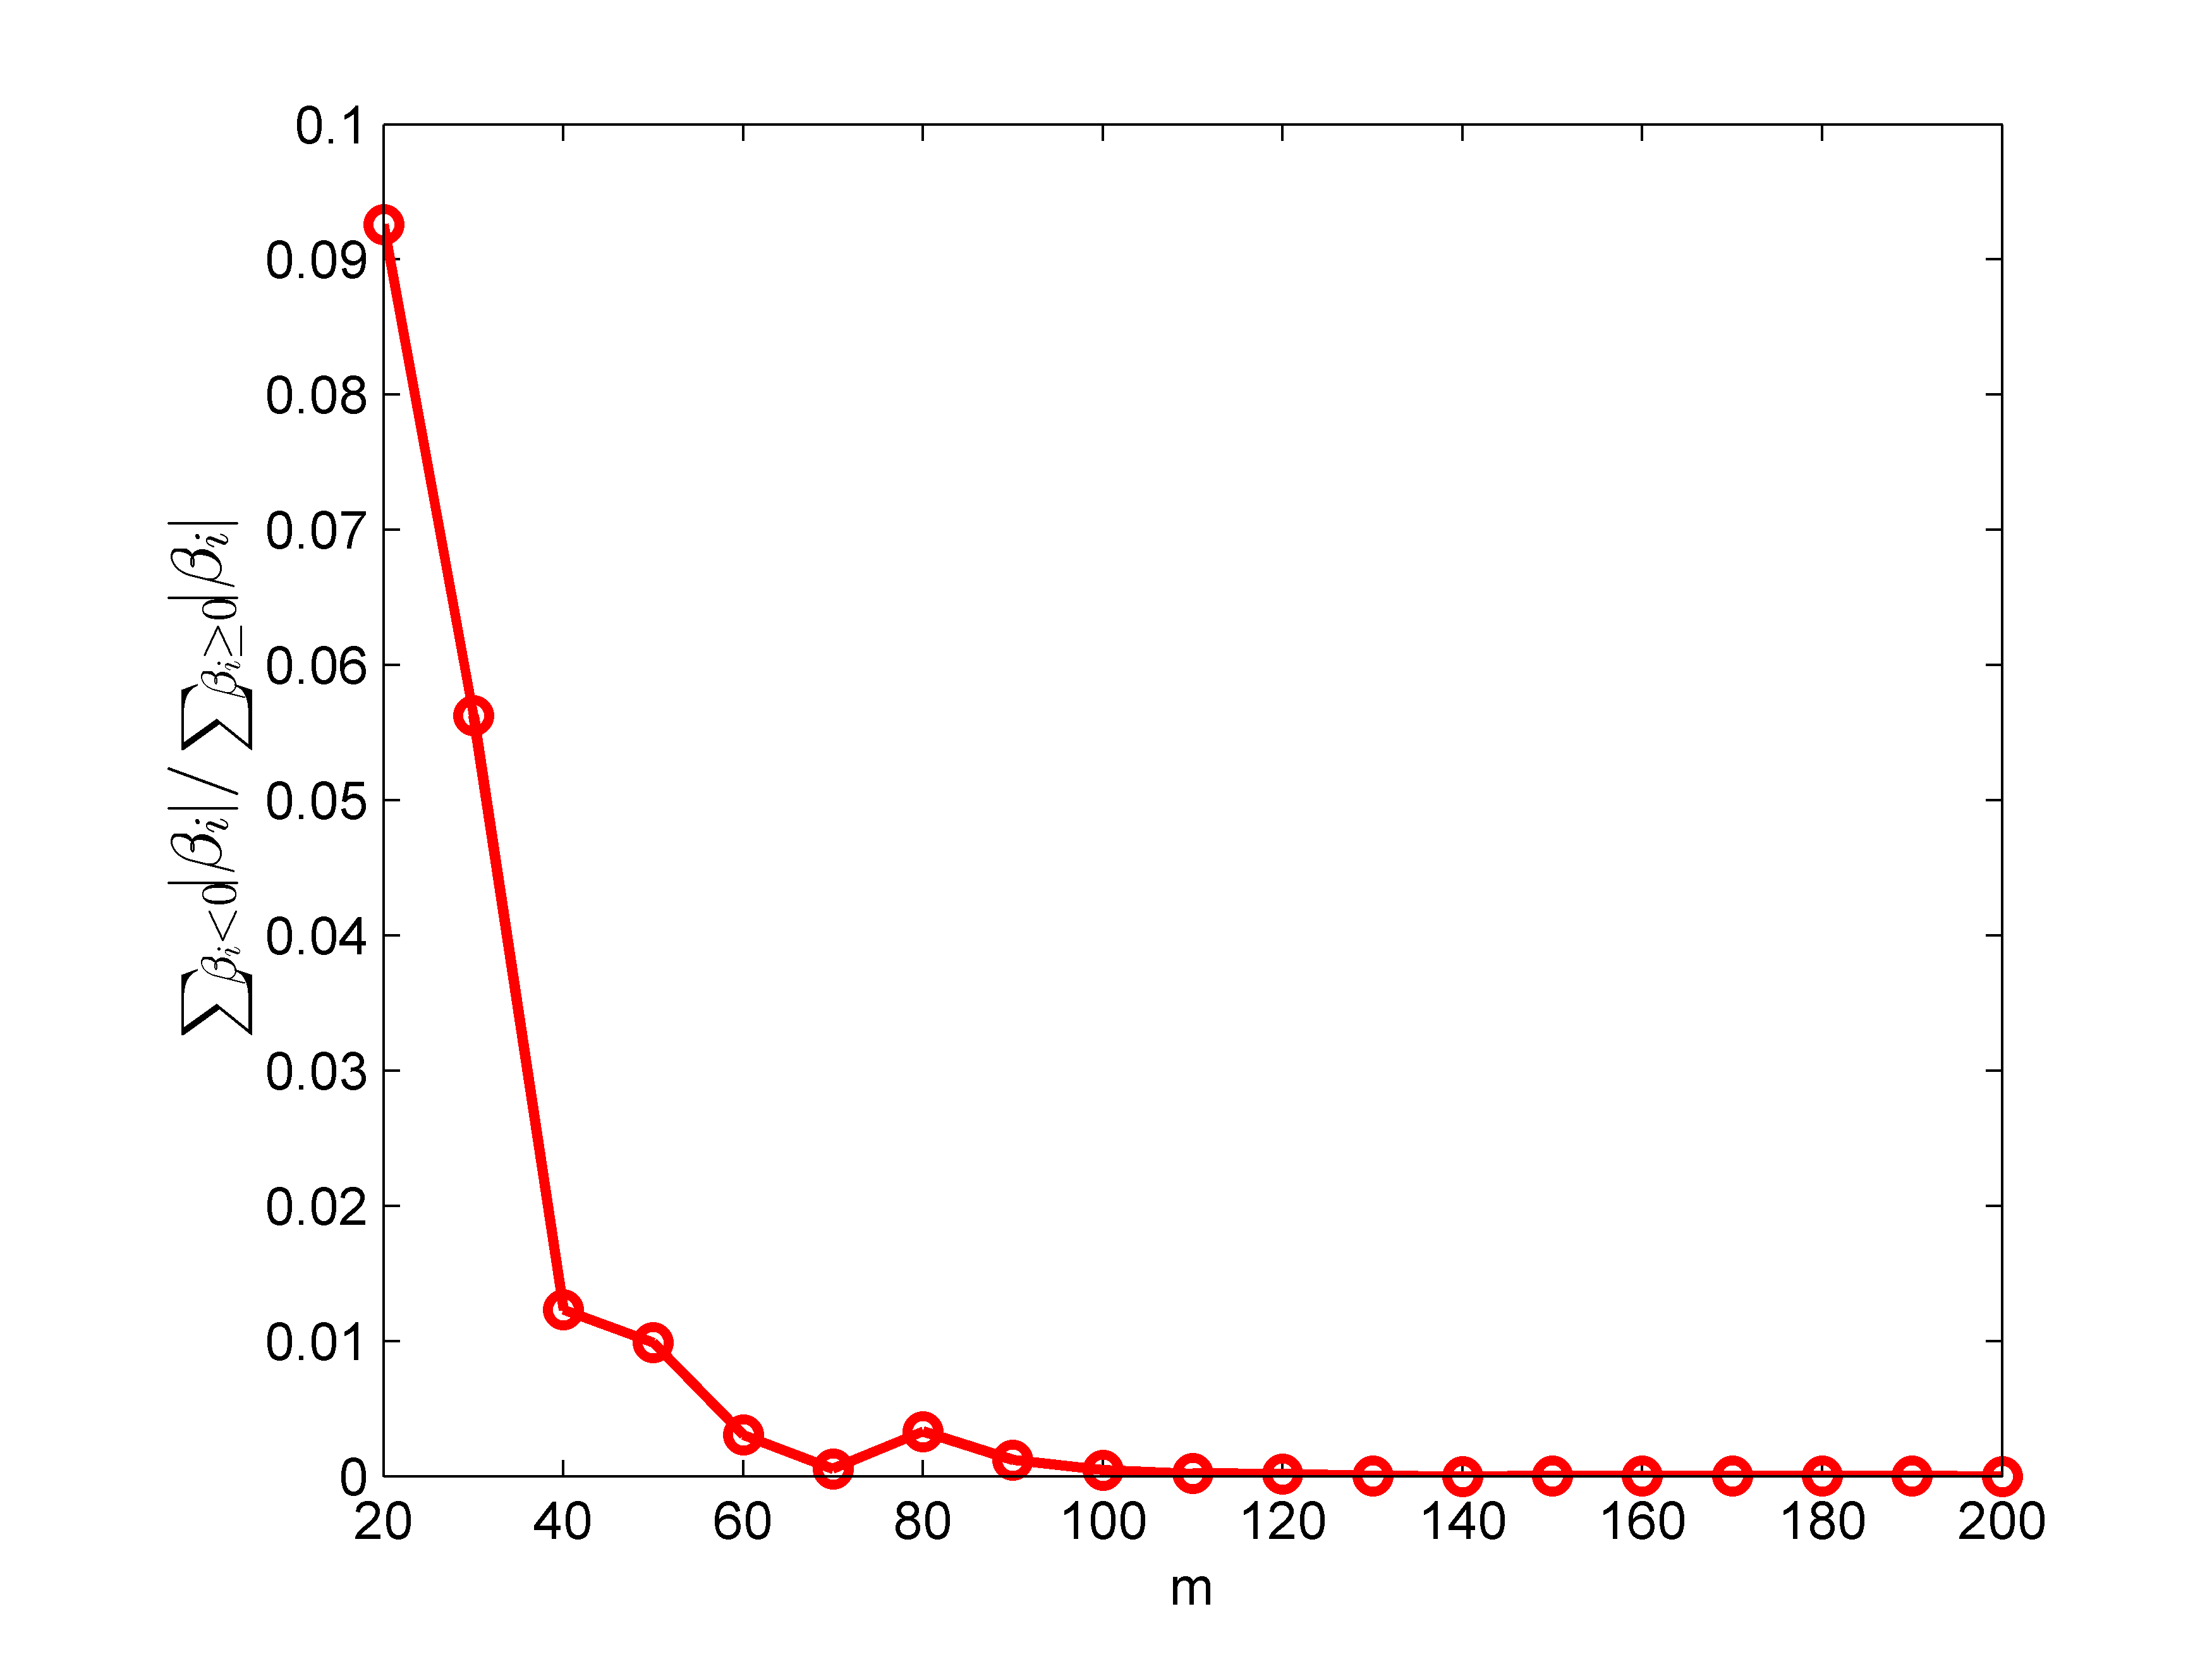
\includegraphics[width=0.6\textwidth]{beta.png}
\end{figure}

\section{Posterior regularized kernel embeddings}
\subsection{Max-Margin Regularization}
We use the hinge loss as an example. Adding the hinge loss regularization to the optimization problem, we get
\begin{align}
\cal{L} = \sum_{i=1}^{m} \beta_i^+ \norm{\phi(y_i) - \mu_{Y|X}^\pi(x_i)}^2 + \lambda\norm{\mu_{Y|X}^\pi}_\Gamma^2 + \mu \sum_{i=m+1}^{n} \max (0, |\langle f, \mu_{Y|X}^\pi(x_i)\rangle_{Y} - t_i| - \epsilon).
\end{align}
Note that $\{(x_1,y_1),(x_2,y_2),\cdots,(x_m,y_m)\}$ is the set of data used to describe the likelihood, while $\{(x_{m+1},t_{m+1}),\cdots,(x_{n},t_{n}) \}$ is the set of data used for supervising posterior regularization.

The good news is that according to Theorem 4.2 in \cite{micchelli2005learning}, the representer theorem still holds for $\cal{L}$. 
\begin{proposition}\label{prop:c}
The solution for $\cal{L}$ has the from $\mu_{Y|X}^\pi(x) = \sum_{i=1}^{n} \Gamma(x,x_i)c_i$, where $c_i \in \cal{H}_Y$ and $\Gamma(x_1,x_2)$ is the reproducing kernel of $\Gamma$. With the choice that $\Gamma(x_1,x_2) = k(x_1,x_2)\cal{I}$ , we have
\begin{align}
c = (K_{xX}\Lambda^+K_{Xx}+\lambda K_{xx})^{-1}\left[K_{xX}\Lambda^+ \Phi + \frac{1}{2}K_{xx}(A^*-A)f\right],\label{eqn:cKinv}
\end{align}
where
\begin{gather}
c = \begin{pmatrix}
c_1\\
c_2\\
\cdots\\
c_{n}
\end{pmatrix},\quad 
f = \begin{pmatrix}
f\\
f\\
\cdots\\
f
\end{pmatrix},\quad
\Phi=\begin{pmatrix}
\phi(y_1)\\
\phi(y_2)\\
\cdots\\
\phi(y_{m})
\end{pmatrix}\\
(K_{Xx})_{i=1:m,j=1:n} = k(x_i,x_j),\quad K_{xX} = K_{Xx}^\T,\quad (K_{xx})_{i=1:n,j=1:n} = k(x_i,x_j)\\
\Lambda^+ = \up{diag}(\beta_1^+,\beta_2^+,\cdots,\beta_m^+)\\
A = \up{diag}(0,\dots,0,\alpha_{m+1},\alpha_{m+2},\cdots,\alpha_{n})\\
A^* = \up{diag}(0,\cdots,0,\alpha_{m+1}^*,\alpha_{m+2}^*,\cdots,\alpha_{n}^*).
\end{gather}

Moreover, the Lagrange multipliers $\alpha_i$ and $\alpha_i^*$ are given by
\begin{gather}
\inf_{\alpha,\alpha^*} \big\{ [\Phi^\T \Lambda^+ K_{Xx} + \frac{1}{2} f^\T (A^* - A)K_{xx}](K_{xX}\Lambda^+ K_{Xx} +\lambda K_{xx})^{-1}[K_{xX}\Lambda^+\Phi + \frac{1}{2} K_{xx} (A^* - A)f]\notag\\- t^\T (\alpha^* - \alpha) + \epsilon 1^\T (\alpha^* + \alpha)\big\}\label{eqn:lagmulti}\\
 s.t.\quad 0 \leq \alpha,\alpha^* \leq \mu,\notag
\end{gather}
where $\alpha = (\alpha_{m+1},\alpha_{m+2},\cdots,\alpha_{n})$, $\alpha^* = (\alpha_{m+1}^*,\alpha_{m+2}^*,\cdots,\alpha_{n}^*)$ and the inequality holds element-wise.
\end{proposition}
\begin{proof}
Apply the representor theorem so that we can reformulate the original problem to be
\begin{align}
\min_{c_i,\xi_i,\xi_i^*}\bigg\{ \sum_{i=1}^m \beta_i^+ \bigg(\phi(y_i) - \sum_{j=1}^{n} k(x_i,x_j)c_j\bigg)^2 + \lambda\bigg(\sum_{i=1}^{n} k_{x_i}c_i\bigg)^2 + \mu \sum_{i=m+1}^{n} (\xi_i + \xi^*_i) \bigg\}
\end{align}
subjected to
\begin{align}
\langle f, \sum_{j=1}^{n} k(x_i,x_j)c_j \rangle - t_i &\leq \epsilon + \xi_i \label{eqn:xi1}\\
t_i - \langle f,\sum_{j=1}^{n} k(x_i,x_j)c_j \rangle &\leq \epsilon + \xi_i^*\label{eqn:xi2}\\
\xi_i, \xi_i^* &\geq 0
\end{align}
We apply the Lagrange duality theory \cite{boyd2004convex} and associate \eqref{eqn:xi1} with $\alpha_i \geq 0$, \eqref{eqn:xi2} with $\alpha_i^* \geq 0$. The Lagrange function is
\begin{align*}
 \cal{L} &= \sum_{i=1}^m \beta_i^+ \bigg(\phi(y_i) - \sum_{j=1}^{n} k(x_i,x_j)c_j\bigg)^2 + \lambda\bigg(\sum_{i=1}^{n} k_{x_i}c_i\bigg)^2 + \mu \sum_{i=m+1}^{n} (\xi_i + \xi^*_i)\\
 &+ \sum_{i=m+1}^{n} \alpha_i (\langle f,\sum_{j=1}^{n} k(x_i,x_j)c_j \rangle - t_i - \epsilon -\xi_i)\\
 &+ \sum_{i=m+1}^{n} \alpha_i^* (t_i - \langle f,\sum_{j=1}^{n} k(x_i,x_j)c_j \rangle - \epsilon - \xi_i^*).
\end{align*}
Now we introduce ad-hoc matrix notations to write $\cal{L}$ in a concise way, where $b^\T A c := \sum_{ij} a_{ij}\langle b_i,c_j\rangle$.
\begin{align}
\cal{L} = c^\T (K_{xX}\Lambda^+ K_{Xx} + \lambda K_{xx})c - (2\Phi^\T \Lambda^+ K_{Xx} + f^\T(A^*-A)K_{xx})c + t^\T (\alpha^* - \alpha) - \epsilon 1^\T (\alpha^* + \alpha) + C.
\end{align}
Note that we implicitly eliminate $\xi_i$ and $\xi_i^*$ by substituting their optimal values. Moreover,
\begin{align}
c^* := \argmin_c \cal{L} = (K_{xX}\Lambda^+K_{Xx}+\lambda K_{xx})^{-1}\left[K_{xX}\Lambda^+ \Phi + \frac{1}{2}K_{xx}(A^*-A)f\right].
\end{align}
where we obtain \eqref{eqn:cKinv}.

Substituting $c^*$ into $\cal{L}$, we can get the optimization problem \eqref{eqn:lagmulti}. 
\end{proof}
This proposition shows that the general solution of this max-margin regularized posterior inference problem $\cal{L}$ is $\mu_{Y|X}(x) = \sum_{i=1}^n \gamma_i(x) \phi(y_i) + \gamma(x) f$. However, if we want to calculate $\mu_{Y|X}(x)$ with numerical methods, we first need to calculate or approximate $\langle f,f \rangle$. This can be easily obtained if $f = \sum_j f_j\phi(y_j')$. For general kernels, such decompositions of any function to sum of feature maps are not trivial. However, finite dimension approximations \cite{rahimi2007random}\cite{oliva2015bayesian} are available to approximate the feature maps of an infinite dimensional RKHS by Schmit orthogonalization. For some special kernels like the Gaussian RBF kernel, we can find an orthnormalized base (ONB) explicitly \cite{steinwart2006explicit}. Both of the approaches can enable us to write $f$ as an expansion of some feature maps, i.e., $f = \sum_{i=1}^{m} f_i\phi(y_i')$.

Another thread is to use \thmref{thm:smola} in case $|\cal{Y}| < \infty$. Since $\langle f, f\rangle_{\cal{H}_Y} = \bf{f}^\T K_Y \bf{f}$, we obtain it! 

The third thread is to treat $\langle f,f\rangle$ as a hyper-parameter, since $f$ is fixed before computing.

\subsubsection{Side note: how to compute $\norm{f}$}
If we already know the value of $f$'s on a fixed set of data points, can we interpolate those data points and compute the norm of the interpolate function? 

\begin{theorem}
Given a set of evaluations $\{(x_1,y_1),(x_2,y_2)\cdots,(x_n,y_n)\}$, and the assumption that evaluation functionals $L_{x_1},L_{x_2},\cdots,L_{x_n}$ are in general position, we can get a function $f \in \cal{H}$ with $f(x_i) = y_i$, and 
%\begin{equation}
%\langle f,f\rangle = \frac{(\bf{y}^\T K^{-1} \bf{y})^2}{\bf{y}^\T (K^2)^{-1}\bf{y}},
%\end{equation}
\begin{equation}
\langle f,f\rangle = \bf{y}^\T K^{-1}\bf{y},
\end{equation}
where $\bf{y} = (y_1,y_2,\cdots,y_n)^\T$ and $K_{ij} = k(x_i,x_j)$.
\end{theorem}
\begin{proof}
Suppose we have $(x_1,y_1),(x_2,y_2),\cdots,(x_n,y_n)$. For each $f \in \cal{H}$, where $\cal{H}$ is a RKHS with kernel function $k(\cdot,\cdot)$, we view $f$ as a functional on $\cal{H}^*$ since $\cal{H}$ is reflective. Under the assumption that evaluation functionals $L_{x_1},L_{x_2},\cdots,L_{x_n}$ are in \textit{general position}, we define $f$ on $\cal{G} = \up{span} \{L_{x_1},L_{x_2},\cdots,L_{x_n}\}$ to be 
\begin{align}
f(\sum_i t_i L_{x_i}) = \sum_i t_i y_i,
\end{align}
where obviously $f(x_i) = y_i$. According to the Hahn-Banach theorem, $f$ can be extended to $\cal{H}$ preserving the norm and values on $\cal{G}$. Now the task is to calculate $\norm{f}_{\cal{G}} = \norm{f}_{\cal{H}}$.

From the definition of norms of functionals, we have that
\begin{align}
\norm{f} &= \sup_{t_{1:n}} \frac{|\sum_i t_i y_i|}{\norm{\sum_i t_i L_{x_i}}}\\
&= \sup_{t_{1:n}} \frac{|\sum_i t_i y_i|}{\sqrt{\sum_{ij} t_i t_j k(x_i,x_j)}}\\
&= \frac{1}{\inf_{t_{1:n}} \sqrt{\sum_{ij} t_i t_j k(x_i,x_j)}}\\
& \quad s.t. \quad \sum_i t_i y_i = 1.
\end{align}
\end{proof}
In order to obtain $\langle f,f\rangle$, we need to solve
\begin{gather*}
\frac{1}{\langle f,f\rangle} = \inf_{t_1,\cdots,t_n} \sum_{i=1}^n\sum_{j=1}^n t_it_j k(x_i,x_j)\\
s.t.\quad \sum_{i=1}^n t_i y_i = 1,
\end{gather*}
which can be solved analytically via Lagrange multipliers to give the result in the theorem.

\subsubsection{Side note: obtaining $f$ via kernel SVM}


\subsection{L2 Regularization}
The regularized optimization problem to study in this section is
\begin{align}
\cal{L} = \sum_{i=1}^{m} \beta_i^+ \norm{\phi(y_i) - \mu_{Y|X}^\pi(x_i)}^2 + \lambda\norm{\mu_{Y|X}^\pi}_\Gamma^2 + \mu \sum_{i=m+1}^{n} \norm{\mu_{Y|X}^\pi(x_i) - \phi(t_i)}^2,
\end{align}
where $\{(x_1,y_1),\cdots,(x_m,y_m)\}$ is the set of samples for estimating the likelihood and the rest is the data for supervising the posterior regularization.
\begin{proposition}
The solution for $\cal{L}$ has the from $\mu_{Y|X}^\pi(x) = \sum_{i=1}^{n} \Gamma(x,x_i)c_i$, where $c_i \in \cal{H}_Y$ and $\Gamma(x_1,x_2)$ is the reproducing kernel of $\Gamma$. With the choice that $\Gamma(x_1,x_2) = k(x_1,x_2)\cal{I}$ , we have
\begin{align}
\muyxplus(x) = \Phi(G_X + \lambda(\Lambda^+)^{-1})^{-1}K_{:x}\label{eqn:l2reg}
\end{align}
where
\begin{align*}
\Phi &= (\phi(Y_1),\phi(Y_2),\cdots,\phi(Y_{n}))\\
K_{:x} &= (K(x,X_1),K(x,X_2),\cdots,K(x,X_{n}))^\T\\
\Lambda^+ &= \up{diag}(\beta_1^+,\beta_2^+,\cdots,\beta_m^+,\mu,\cdots,\mu).
\end{align*}
\end{proposition}
\begin{proof}
The proof is analogous to that of \propref{prop:bayes+}.
\end{proof}
\section{Kernel Posterior Average and Posterior Decoding}
There are some tweaks for obtaining estimations of the posterior average and the MAP value compared to \cite{song2013kernel}, since we introduce $f$ in the expression of kernel posterior embedding. After obtaining the estimation of kernel regularized posterior $\mu_{Y|X}^\pi(x) = \sum_{i=1}^n \gamma_i(x) \phi(y_i) + \gamma(x) f$, the average of any other function $g$ should be computed as $\langle g, \mu_{Y|X}^\pi(x)\rangle = \sum_{i=1}^{n} \gamma_i(x)g(y_i) + \gamma(x) \langle g,f\rangle$, and the MAP value can obtained by finding the closest kernel mapping to the kernel posterior regularized embedding, i.e., $\hat{y} = \argmax_{y} \|\mu_{Y|X}^\pi(x) - \phi(y)\|^2 = \argmin_{y} \{ %\sum_{ij}\gamma_i(x)\gamma_j(x)k(y_i,y_j) + 2\sum_i \gamma_i(x)\gamma(x)f(y_i) %+ \gamma^2(x)\langle f,f\rangle 
- 2\sum_i\gamma_i(x)k(y_i,y) - 2\gamma(x)f(y) + k(y,y)\}$. 

The main difficulty here is still finding $\langle f,g\rangle$ and $\langle f,f\rangle$. As discussed before, in finite state space case, we may use $\langle f,g\rangle = \bf{f}^\T K_Y \bf{g}$.
\section{Proof for Consistency of $(\widehat{\mu}_Z^{\pi})^+$}
Recap: $(\widehat{\mu}_Z^{\pi})^+ = \sum_{i=1}^m \beta_i^+\varphi(Z_i) $. We already know that $\widehat{\mu}_Z^\pi = \sum_{i=1}^m \beta_i \varphi(Z_i) = \widehat{C}_{ZY}(\widehat{C}_{YY}+\lambda_m I)^{-1} \widehat{\pi}_Y$ convergences to $C_{ZY}C_{YY}^{-1}\pi_Y = \mu_Z^\pi$ in probability.

The consistency of $(\widehat{\mu}_Z^\pi)^+$ can be proved under the condition that $|\cal{Z}| < \infty$. The proof was inspired by \cite{grunewalder2012modelling}. We first introduce an auxiliary result from \cite{smola2003kernels}.
\begin{theorem}[\cite{smola2003kernels}, Thm. 4]\label{thm:smola}
Denote by $P\in \mathbb{R}^{m\times m}$ a (positive semidefinite) regularization matrix and denote by $\mathcal{H}$ the image of $\bb{R} ^m$ under $P$. Then $\mathcal{H}$ with dot product $\langle f, f\rangle_{\cal{H}} := \langle \bf{f}, P\bf{f}\rangle$ is a Reproducing Kernel Hilbert Space and its kernel is $k(i,j) = P^+_{ij}$, where $P^+$ is the pseudo-inverse of $P$.
\end{theorem}

\begin{theorem}\label{thm:main}
Assume that $|\cal{Z}| = |\cal{X}\times\cal{Y}| < \infty$, $k_Z$ is a bounded kernel with $k_Z(Z,Z) \leq K$ for all $Z$, $C_{YY}$ is injective, $\widehat{\pi}_Y$ is a consistent estimator of $\pi_Y$ in $\cal{H}_Y$ norm, the observed data $\cal{Z} = \{ (x_1,y_1),(x_2,y_2),\cdots,(x_n,y_n) \}$ are linear independent and that $\bb{E}[k_Z(Z,\tilde{Z})\mid Y=y,\tilde{Y}=\tilde{y}]$ is included in $\cal{H}_Y \otimes \cal{H}_Z$ as a function of $(y,\tilde{y})$. Then, if the regularization coefficient $\lambda_n$ decays to zero sufficiently slowly,
\begin{align}
\norm{(\widehat{\mu}_Z^{\pi})^+ - \mu_Z^\pi}_{\cal{H}_Z} \rightarrow 0 
\end{align}
in probability as $n\rightarrow\infty$.
\end{theorem}
\begin{proof}
From Theorem 8 in \cite{fukumizu2011kernel} we already know that $\norm{\widehat{\mu}_Z^\pi-\mu_Z^\pi}_{\cal{H}_Z} \rightarrow 0$ in probability. Thus the theorem can be proved if $\norm{(\widehat{\mu}_Z^{\pi})^+ - \widehat{\mu}_Z^\pi}_{\cal{H}_Z} \rightarrow 0$. 

In this proof we assume that $|\cal{Z}| = n$ and the sample size is $m$. For brevity and without losing generality, we assume $\cal{Z} = \{ (x_1,y_1),\cdots,(x_n,y_n) \}$ and $\{ (x_1,y_1),\cdots,(x_m,y_m) \}$ is an observed sample to be considered. Because $k_Z$ is positive definite on a finite set, \thmref{thm:smola} shows that $\cal{H}_Z$ consists of all bounded functions on $\cal{Z} = \{ (x_1,y_1),(x_2,y_2),\cdots,(x_n,y_n) \}$ and $\langle f,g\rangle_{\cal{H}_Z} = \bf{f}^\T R^+ \bf{g}$, where $R = (k_Z(z_i,z_j))_{i,j=1}^n$ and $\bf{f}:=(f(x_i,y_i))_{i=1}^n$ is the vector of point evaluations of $f$ on $\cal{Z}$. In particular, $\cal{H}_Z$ contains the function
\begin{align}
f(z_i) = \begin{cases}
1, \quad &\beta_i < 0\\
0,\quad &\text{$\beta_i \geq 0$ or $z_i$ is not observed in this sample}
\end{cases}
\end{align}
Since $|\cal{Z}|<\infty$, the number of different $f$ is limited and thus we can denote $\max_f \norm{f}_{\cal{H}_Z} = b$.

From the non-negativity we have $\bb{E}[f(Z)] \geq 0$. Due to the consistency of $\widehat{\mu}_Z^\pi$, we have $|\langle \widehat{\mu}_Z^\pi, f\rangle - \langle \mu_Z^\pi, f\rangle| \leq \norm{\widehat{\mu}_Z^\pi-\mu_Z^\pi}_{\cal{H}_Z}\norm{f}_{\cal{H}_Z} < \epsilon\norm{f}_{\cal{H}_Z}$. Note that $f$ is specially designed to let $\langle \widehat{\mu}_Z^\pi ,f\rangle = - \sum_{i=1}^m \beta_i^-$, where $\beta_i^- = -\min(0,\beta_i)$. Combined with the fact $\langle \mu_Z^\pi,f\rangle \geq 0$, we obtain
\begin{align}
\sum_{i=1}^m \beta_i^- < \epsilon \norm{f}_{\cal{H}_Z}.
\end{align}

On the other hand, we have
%We consider a non-negative function $f:Z\rightarrow\bb{R}$ as described below:
%\begin{align}
%f(Z) = \begin{cases}
%a,\quad Z \leq 0\\
%0,\quad Z > 0,
%\end{cases}
%\end{align}
%where we choose $a$ to be a sufficiently large fixed number. Since $\cal{H}_Z$ is an RKHS with a universal kernel, for every $\delta > 0$, there is a function $h\in \cal{H}_Z:Z \rightarrow \bb{R} $ with $|h(Z) - f(Z)| < \delta$ for all $Z$. From $h(Z) \geq -\delta$, we know $\bb{E}_Z(h(Z)) \geq -\delta$, which is the same as $\langle \mu_Z^\pi , h \rangle \geq -\delta$. 

%From Cauchy-Schwartz inequality, we know
%\begin{align}
%&|\langle \widehat{\mu}_Z^\pi, h\rangle - \langle \mu_Z^\pi, h\rangle |\\
%=&|\langle \widehat{\mu}_Z^\pi - \mu_Z^\pi, h\rangle |\\
%\leq& \norm{\widehat{\mu}_Z^\pi - \mu_Z^\pi}_{\cal{H}_Z}\cdot \norm{h}_{\cal{H}_Z}
%\end{align}
%According to the definition of convergence in probability, we know $\forall \epsilon>0$, $\norm{\widehat{\mu}_Z^\pi - \mu_Z^\pi}_{\cal{H}_Z} < \epsilon$ holds with arbitrary high probability as long as $n$ is sufficiently large. In this case $|\langle \widehat{\mu}_Z^\pi, h\rangle - \langle \mu_Z^\pi, h\rangle | \leq \epsilon \norm{h}_{\cal{H}_Z} $. Combining this fact with $\sup|h-f|<\delta$, we obtain
%\begin{align}
%&\langle \widehat{\mu}_Z^\pi ,h \rangle \geq -\delta - \epsilon \norm{h}\\
%\Rightarrow& \sum_{i=1}^n \beta_i^+ \delta - \sum_{i=1}^n \beta_i^-(a - \delta) \geq -\delta - \epsilon\norm{h}\\
%\Rightarrow& \sum_{i=1}^{n} \beta_i^-  \leq \frac{\delta + \epsilon\norm{h} + \sum_{i=1}^n \beta_i^+ \delta}{a-\delta},
%\end{align}
%where $\beta_i^- = -\min(0,\beta_i)$. With this inequality we can bound the difference between $(\widehat{\mu}_Z^\pi)^+$ and $\widehat{\mu}_Z^\pi$,

\begin{align}
\norm{(\widehat{\mu}_Z^\pi)^+ - \widehat{\mu}_Z^\pi}_{\cal{H}_Z} &= \norm{\sum_{i=1}^m\beta_i^- \varphi(Z_i)}\\
&= \sqrt{\sum_{i,j} \beta_i^-\beta_j^- k(Z_i,Z_j) }\\
&\leq \sqrt{K} \sum_{i=1}\beta_i^-\\
&<  \epsilon\sqrt{K} \norm{f}_{\cal{H}_Z}\\
&<  \epsilon\sqrt{K}b,
\end{align}
which means $(\widehat{\mu}_Z^\pi)^+ \rightarrow \widehat{\mu}_Z^\pi$ in probability.

Moreover, we can relate $b$ and the number of samples $m$ in the following way
\begin{align}
 \norm{f}_{\cal{H}_Z} = \sqrt{\bf{f}^\T R^+ \bf{f}} \leq \sqrt{m^2 K} = m\sqrt{K}.
\end{align}
As a result,
\begin{equation}
\norm{(\widehat{\mu}_Z^\pi)^+ - \widehat{\mu}_Z^\pi}_{\cal{H}_Z} < \epsilon m K.
\end{equation}
\end{proof}
\begin{remark}
When $|\cal{Z}| = n$, we always have $\norm{f}_{\cal{H}_Z} \leq n\sqrt{K}$ and $\norm{(\widehat{\mu}_Z^\pi)^+ - \widehat{\mu}_Z^\pi}_{\cal{H}_Z} < \epsilon n K$ and thus $(\widehat{\mu}_Z^\pi)^+$ always converges. Under all needed assumptions, the best provable and achievable convergence rate demonstrated in \cite{fukumizu2011kernel} is $\epsilon = O_p(m^{-\frac{1}{2}})$. For this reason $(\widehat{\mu}_Z^\pi)^+$ is not guaranteed to convergence in the case $|\cal{Z}| = \infty$.
\end{remark}
\begin{remark}
\thmref{thm:main} establishes the convergence of the operator used in \cite{nishiyama2012hilbert}, which was posted as an open problem.
\end{remark}
\begin{remark}
We can use $(\widehat{\mu}_Z^\pi)^+$ as an approximation when $|\cal{Z}| = \infty$, though the convergence remains unexamined. Empirically this approximation works especially well when the prior and posterior distributions are similar.
\end{remark}
\begin{remark}
Another ad hoc method is to use $\beta$ directly instead of $\beta^+$ when $|\cal{Z}| = \infty$. Although this will make the optimization problem non-convex and even do not have minima, we can use it as an approximation. There are examples where people use techniques developed and proved for convex problems to non-convex optimization, such as deep neural network training methods \cite{nesterov1983method}\cite{duchi2011adaptive}. ({\color{red}remains to be examined by experiments})
\end{remark}
\section{Normalization}
For implementation purpose, we usually normalize a kernel mean estimator for numerical stability.
\begin{theorem}
Suppose $\cal{H}$ is a RKHS with a universal kernel. If $\bar{u} = \sum_{i=1}^n \beta_i \phi(x_i)$ is a consistent estimator for a kernel mean $\mu$ in $\cal{H}$, then the normalized estimator
\begin{align}
\hat{\mu} = \sum_{i=1}^n \hat{\beta}_i \phi(x_i)
\end{align}
where $\hat{\beta}_i = \frac{\beta_i}{\sum_{i=1}^n \beta_i}$ is also a consistent estimator for $\mu$.
\end{theorem}
\begin{proof}
Since $\cal{H}$ is dense in $C_0(\cal{X})$, we can choose a sequence of functions $\{f_1,f_2,\cdots,f_n,\cdots\}, f_i \in \cal{H}$ which uniformly converges to the constant $1$. 
\end{proof}
{\color{red} I cannot finish the proof here. It seems that this can only hold for discrete cases. Also empirically it's not necessary to normalize the kernel means if the parameters are appropriate.}
\section{Experiments}
\subsection{Kernel Filtering}
\paragraph{Training:}
Following the settings in \cite{fukumizu2011kernel}, we assume a sample $(Y_1,X_1,\cdots,Y_{T+1},X_{T+1})$ is given. Presuming homogeneity of the HMM, we can use empirical covariance operators to estimate the transition and observation probabilities in a nonparametric way:
\begin{align}
\hat{C}_{YX} &= \frac{1}{T}\sum_{i=1}^T \phi(Y_i)\otimes\psi(X_i),\quad \hat{C}_{YY_+} = \frac{1}{T}\sum_{i=1}^T \phi(Y_{i})\otimes \phi(Y_{i+1})\\
\hat{C}_{XX} &= \frac{1}{T}\sum_{i=1}^T \psi(X_i) \otimes \psi(X_i),\quad \hat{C}_{YY} = \frac{1}{T}\sum_{i=1}^T \phi(Y_i)\otimes\phi(Y_i).
\end{align}
\paragraph{Filtering:}
Now we can derive recursive formulas for the state-space filtering task. Suppose we already have an estimator of the embedding for $p(y_t|x_1,\cdots,x_t)$ in the form
\begin{align}
\hat{m}_{y_t|x_1,\cdots,x_t} = \sum_{i=1}^T \alpha_i^{(t)} \phi(Y_i).
\end{align}
The update rule for $\alpha^{(t+1)}(x_1,\cdots,x_{t+1})$ can be derived by a prediction and a correction step. For the forward propagation, we have the following empirical estimators,
\begin{align}
\hat{m}_{y_{t+1}\mid x_1,\cdots,x_t} &= \hat{C}_{Y_{+}Y}(\hat{C}_{YY}+\lambda_T I)^{-1}\hat{m}_{y_t\mid x_1,\cdots,x_t} = \Phi_{+}(G_Y + T\lambda_T I)^{-1}G_Y \alpha^{(t)}\\
\hat{m}_{x_{t+1}\mid x_1,\cdots,x_t} &= \hat{C}_{XY}(\hat{C}_{YY} + \lambda_{T}I)^{-1}\hat{m}_{y_{t+1}|x_1,\cdots,x_t} = \Psi(G_{Y} + T\lambda_T I)^{-1} G_{YY_+}(G_Y + T\lambda_T I)^{-1}G_{Y} \alpha^{(t)},
\end{align}
where $\hat{m}_{x_{t+1}\mid x_1,\cdots,x_t}$ is the embedding for prediction. According to \eqref{eqn:bayes}, we can obtain $\hat{m}_{y_{t+1}\mid x_1,\cdots,x_{t+1}}$ easily,
\begin{align}
&\hat{m}_{y_{t+1}\mid x_1,\cdots,x_{t+1}} = \Phi(K_X + \delta_T (\Lambda^+)^{-1})^{-1} K_{:x_{t+1}},\\
\Leftrightarrow& \alpha^{(t+1)} = (K_X + \delta_T (\Lambda^+)^{-1})^{-1} K_{:x_{t+1}}
\end{align}
where $\Lambda^+ = \up{diag}(\bs{\beta}^+)$ and $\bs{\beta} = (G_Y + T\lambda_T I)^{-1}G_{YY+}(G_Y + T\lambda_T I)^{-1}G_Y \alpha^{(t)}$.

For an initial estimate, we use conditional kernel embedding $\widehat{C}_{YX}(\widehat{C}_{YX} + \lambda_n I)^{-1} K_{:x_1}$, yielding $\alpha^{(1)} = T(K_X + T\lambda_T I)^{-1}K_{:x_1}$.

\paragraph{L2 Regularized Filtering}
Ignoring process noise and observation noise, we assume that the states and observations of the dynamics should be $(\tilde{Y}_1,\tilde{X}_1,\cdots,\tilde{Y}_N,\tilde{X}_N)$. Here we assume instead that 
\begin{align}
\hat{m}_{y_t|x_1,\cdots,x_t} = \sum_{i=1}^T \alpha_i^{(t)} \phi(Y_i) + \sum_{i=1}^N \tilde{\alpha}_i^{(t)} \phi(\tilde{Y}_i)
\end{align}
Similar to what we did before,
\begin{align}
\hat{m}_{y_{t+1}\mid x_1,\cdots,x_t} &= \hat{C}_{Y_{+}Y}(\hat{C}_{YY}+\lambda_T I)^{-1}\hat{m}_{y_t\mid x_1,\cdots,x_t} \\
&= \Phi_{+}G_{Yy}(G_{yY}G_{Yy} + T\lambda_T G_{yy})^{-1}G_{yy} \begin{pmatrix}
\alpha^{(t)}\\
\tilde{\alpha}^{(t)}
\end{pmatrix}\\
\hat{m}_{x_{t+1}\mid x_1,\cdots,x_t} &= \hat{C}_{XY}(\hat{C}_{YY} + \lambda_{T}I)^{-1}\hat{m}_{y_{t+1}|x_1,\cdots,x_t} \\
&= \Psi(G_{Y} + T\lambda_T I)^{-1} G_{YY_+}G_{Yy}(G_{yY}G_{Yy} + T\lambda_T G_{yy})^{-1}G_{yy} \begin{pmatrix}
\alpha^{(t)}\\
\tilde{\alpha}^{(t)}
\end{pmatrix},
\end{align}
where $(G_{YY})_{ij} = K(Y_i,Y_j)$,
$
G_{Yy} = \begin{pmatrix}
G_{YY}, G_{Y\tilde{Y}}
\end{pmatrix}
$,$G_{yY} = G_{Yy}^\T$ and $G_{yy} = \begin{pmatrix}
G_{YY} & G_{Y\tilde{Y}}\\
G_{\tilde{Y}Y} & G_{\tilde{Y}\tilde{Y}}
\end{pmatrix}$.

For the update rule of the $t$ step, we solve the optimization problem
\begin{align}
\cal{L} = \sum_{i=1}^{m} \beta_i^+ \norm{\phi(y_i) - \mu_{Y|X}^\pi(x_i)}^2 + \delta_T\norm{\mu_{Y|X}^\pi}_\Gamma^2 + \mu_T \norm{\mu_{Y|X}^\pi(\tilde{x}_t) - \phi(t_t)}^2,
\end{align}
where $t_t$ is the state at the $t$ step according to the dynamics without noise and $\tilde{x}_t$ is the observation of $t_t$ according to the observation model without noise. Exploiting \eqref{eqn:l2reg}, we obtain $\hat{m}_{y_{t+1}\mid x_1,\cdots,x_{t+1}}$,
\begin{align}
&\hat{m}_{y_{t+1}\mid x_1,\cdots,x_{t+1}} = \Phi(K_X' + \delta_T (\Lambda^+)^{-1})^{-1} K_{:x_{t+1}}',\\
\Leftrightarrow& \alpha^{(t+1)} = (K_X' + \delta_T (\Lambda^+)^{-1})^{-1} K_{:x_{t+1}}'
\end{align}
where $\Lambda^+ = \up{diag}(\bs{\beta}^+,\mu_T)$, $\bs{\beta} = (G_Y + T\lambda_T I)^{-1}G_{YY_+}G_{Yy}(G_{yY}G_{Yy} + T\lambda_T G_{yy})^{-1}G_{yy} \begin{pmatrix}
\alpha^{(t)}\\
\tilde{\alpha}^{(t)}
\end{pmatrix}$ and $K_X'$ and $K_{:x_{t+1}}'$ incorporates $K(\tilde{x}_{t+1},\cdot)$.
\paragraph{Max-Margin Filtering:} We assume that 
\begin{align}
\hat{m}_{y_t|x_1,\cdots,x_t} = \sum_{i=1}^T \alpha_i^{(t)} \phi(Y_i) + \beta^{(t)} f.
\end{align}
With similar calculations, we obtain the prediction step of the filter:
\begin{align}
\hat{m}_{y_{t+1}\mid x_1,\cdots,x_t} &= \hat{C}_{Y_{+}Y}(\hat{C}_{YY}+\lambda_T I)^{-1}\hat{m}_{y_t\mid x_1,\cdots,x_t} \\
&= \Phi_+^\T (G_Y + T \lambda_T I)^{-1} (G_Y\alpha^{(t)} + \beta^{(t)}f_{1:T}),
\end{align}
where $f_{1:T} = (f(Y_1),f(Y_2),\cdots,f(Y_T))^\T$ and $\alpha^{(t)} = (\alpha_1^{(t)},\alpha_2^{(t)}\cdots,\alpha_T^{(t)})^\T$. The weights $\bs{\beta}$ can be calculated as
\begin{align}
\bs{\beta} = (G_Y + T\lambda_T I)^{-1}G_{YY_+}(G_Y + T \lambda_T I)^{-1} (G_Y\alpha^{(t)} + \beta^{(t)}f_{1:T}).
\end{align}

For the update phase of the filter, we need to solve the optimization problem
\begin{align}
\cal{L} = \sum_{i=1}^{m} \beta_i^+ \norm{\phi(y_i) - \mu_{Y|X}^\pi(x_i)}^2 + \delta_T\norm{\mu_{Y|X}^\pi}_\Gamma^2 + \mu_T \max (0, |\langle f, \mu_{Y|X}^\pi(x_t)\rangle_{Y} - t_t| - \epsilon),
\end{align}
where $x_t$ is the observation at the $t$ step and $t_t$ is the value that we expect the expectation of $f$ w.r.t. the hidden state at the $t$ step to have.
The update rules for the filter are
\begin{align}
\alpha^{(t+1)} &= \Lambda^+ K_{Xx}(K_{xX}\Lambda^+K_{Xx}+\delta_T K_{xx})^{-1}K_{:x_{t+1}}\\
\beta^{(t+1)} &= \frac{1}{2} \bf{1}^\T (A^*-A) K_{xx}(K_{xX}\Lambda^+K_{Xx}+\delta_T K_{xx})^{-1}K_{:x_{t+1}},
\end{align}
where $\alpha$ and $\alpha^*$ need to be solved from
\begin{gather}
\inf_{\alpha,\alpha^*} \big\{ [\Phi^\T \Lambda^+ K_{Xx} + \frac{1}{2} f^\T (A^* - A)K_{xx}](K_{xX}\Lambda^+ K_{Xx} +\delta_T K_{xx})^{-1}[K_{xX}\Lambda^+\Phi + \frac{1}{2} K_{xx} (A^* - A)f]\notag\\- t_t(\alpha^* - \alpha) + \epsilon  (\alpha^* + \alpha)\big\}\\
 s.t.\quad 0 \leq \alpha,\alpha^* \leq \mu_T.\notag
\end{gather}

\paragraph{Posterior Decoding:} The kernel means for the states can always be written as $\hat{m}_{y_t|x_1,\cdots,x_t} = \sum_{i=1}^T \alpha_i^{(t)}\phi(Y_i)$. As before, the optimization problem $\hat{Y}_i = \argmin_{y}\norm{\sum_{i=1}^T \alpha_i^{(t)}\phi(Y_i) - \phi(y)}^2$ yields $\hat{Y}_i = \argmin_y \{ k(y,y) - 2\sum_{i=1}^T \alpha_i^{(t)}k(y_i,y)\}$. For Gaussian kernel, there is a fixed point iteration method which empirically converges fast:
\begin{align}
y^{(n+1)} = \frac{\sum_{i=1}^T Y_i \alpha_i^{(t)}\exp(-\norm{Y_i-y^{(n)}}^2/(2\sigma^2))}{\sum_{i=1}^T \alpha_i^{(t)}\exp(-\norm{Y_i-y^{(n)}}^2/(2\sigma^2))}.
\end{align}
To decode the kernel mean derived from max-margin kernel filtering, we need to slightly adapt the above iteration rule to be
\begin{align}
y^{(n+1)} = \frac{\sum_{i=1}^T Y_i\alpha_i^{(t)}\exp(-\norm{Y_i-y^{(n)}}^2/(2\sigma^2)) + \sigma^2 \beta^{(t)} f'(y^{(n)}) }{\sum_{i=1}^T\alpha_i^{(t)} \exp(-\norm{Y_i-y^{(n)}}^2/(2\sigma^2))}.
\end{align}
\bibliography{note.bib}
\end{document}